\documentclass[11pt]{article}

\usepackage[margin=0.8in]{geometry}
\usepackage[T1]{fontenc}
\usepackage{lmodern}
\usepackage{xcolor}
\usepackage{array}
\usepackage{booktabs}
\usepackage{longtable}
\usepackage{tabularx}
\usepackage{enumitem}
\usepackage{listings}
\usepackage{tikz}
\usepackage{hyperref}
\usepackage{titlesec}
\usepackage{fancyhdr}

\usetikzlibrary{arrows.meta,backgrounds,calc,fit,positioning,shadows.blur,shapes.geometric}

\definecolor{prismblue}{HTML}{2457A6}
\definecolor{prismcyan}{HTML}{1D9AAB}
\definecolor{prismgreen}{HTML}{2E8B57}
\definecolor{prismorange}{HTML}{E6862F}
\definecolor{prismpurple}{HTML}{7562C8}
\definecolor{prismred}{HTML}{C94C4C}
\definecolor{prismgray}{HTML}{F4F6FA}
\definecolor{darkgray}{HTML}{333B4F}

\hypersetup{
  colorlinks=true,
  linkcolor=prismblue,
  urlcolor=prismpurple,
  citecolor=prismgreen
}

\pagestyle{fancy}
\fancyhf{}
\lhead{Intelligent Multimodal RAG Platform}
\rhead{Product \& Technical Roadmap}
\cfoot{\thepage}
\renewcommand{\headrulewidth}{0.4pt}

\titleformat{\section}{\Large\bfseries\color{prismblue}}{}{0pt}{}
\titleformat{\subsection}{\large\bfseries\color{prismpurple}}{}{0pt}{}
\titleformat{\subsubsection}{\bfseries\color{darkgray}}{}{0pt}{}

\setlength{\parindent}{0pt}
\setlength{\parskip}{0.55\baselineskip}
\setlength{\headheight}{14pt}
\setlist[itemize]{leftmargin=1.4em,itemsep=0.2em,topsep=0.2em}
\setlist[enumerate]{leftmargin=1.6em,itemsep=0.2em,topsep=0.2em}
\renewcommand{\arraystretch}{1.25}

\lstdefinestyle{roadmapcode}{
  basicstyle=\ttfamily\small,
  backgroundcolor=\color{prismgray},
  frame=single,
  rulecolor=\color{prismblue!30},
  breaklines=true,
  columns=fullflexible,
  keepspaces=true,
  showstringspaces=false
}
\lstset{style=roadmapcode}

\newcolumntype{Y}{>{\raggedright\arraybackslash}X}

\tikzset{
  block/.style={rectangle,rounded corners=5pt,draw=#1!80,fill=#1!12,very thick,
    minimum width=3.2cm,minimum height=0.9cm,align=center,font=\small\bfseries,blur shadow},
  block/.default=prismblue,
  smallblock/.style={rectangle,rounded corners=4pt,draw=#1!80,fill=#1!12,thick,
    minimum width=2.45cm,minimum height=0.8cm,align=center,font=\scriptsize\bfseries},
  smallblock/.default=prismblue,
  store/.style={cylinder,shape border rotate=90,aspect=0.25,draw=#1!85,fill=#1!12,very thick,
    minimum width=2.7cm,minimum height=1.1cm,align=center,font=\small\bfseries,blur shadow},
  store/.default=prismgreen,
  arrow/.style={-{Latex[length=2.4mm]},very thick,draw=darkgray!80},
  faintarrow/.style={-{Latex[length=2.1mm]},thick,draw=darkgray!55},
  group/.style={rounded corners=8pt,draw=#1!55,fill=#1!5,thick,inner sep=8pt},
  group/.default=prismblue
}

\title{\bfseries\color{prismblue}MultiAgent RAG Platform for SBI\\[-0.2em]}
\date{\today}

\begin{document}
\maketitle


\subsection{Retrieval Strategy Matches Data Type}
\begin{table}[h]
\centering
\begin{tabularx}{\textwidth}{>{\bfseries}lY}
\toprule
Data Type & Retrieval Strategy \\
\midrule
CSV / Excel & TableRAG \\
PDF & Hierarchical Structure-Aware RAG \\
Markdown & Structure-Aware RAG \\
Plain Text & Vector RAG \\
Government Schemes Database & SQL Retrieval \\
External Websites & Web Retrieval Agent \\
Voice Queries & Speech-to-RAG Pipeline \\
\bottomrule
\end{tabularx}
\caption{Document-type-specific retrieval strategies.}
\end{table}

\subsection{Metadata-First Architecture}
Every document, chunk, embedding, and retrieval operation preserves rich metadata.
Metadata quality often contributes more to retrieval accuracy than embedding model
selection, especially when users ask questions scoped by file, state, language,
section, or source.

\section{Goal 1: Canonical Government Schemes Data Platform}

\subsection{Objective}
Create a normalized repository of government scheme information stored in SQLite with
APIs and frontend access.

\subsection{Methodology}
Government scheme datasets often contain inconsistent field names, duplicated records,
and varying structures. The ingestion layer normalizes column names, state names,
scheme identifiers, ministry names, URLs, and dates into a canonical schema.

\begin{lstlisting}[language=SQL,caption={Canonical scheme fields.}]
scheme_id
scheme_name
state
ministry
department
eligibility
benefits
application_process
required_documents
official_website
source_url
last_updated
\end{lstlisting}

SQLite indexes should cover \texttt{scheme\_name}, \texttt{state}, and
\texttt{ministry}. The API exposes list, filter, and detail endpoints.

\begin{lstlisting}[caption={Scheme API endpoints.}]
GET /schemes
GET /schemes?state=Karnataka
GET /schemes?name=PM Kisan
GET /schemes/{id}
\end{lstlisting}

The frontend displays canonical fields, official links, related schemes, source
documents, and retrieval sources. Success means sub-second lookup, a consistent schema,
and reliable SQL retrieval.

\section{Goal 2: Intelligent Upload and Strategy Selection}

\subsection{Objective}
Allow users to upload files and automatically determine the best embedding and retrieval
strategy. Supported types include CSV, Excel, PDF, Markdown, Word, HTML, plain text, and
audio.

\begin{figure}[h]
\centering
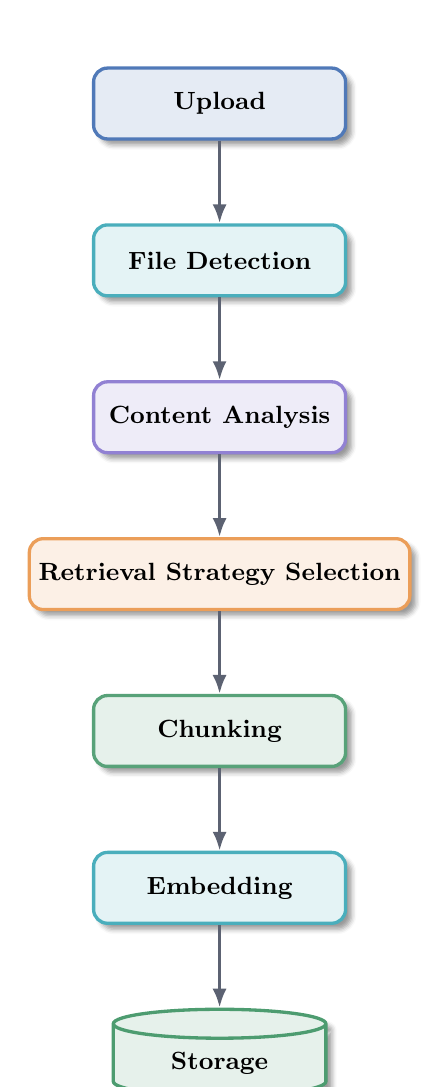
\begin{tikzpicture}[node distance=1.05cm]
\node[block=prismblue] (upload) {Upload};
\node[block=prismcyan,below=of upload] (detect) {File Detection};
\node[block=prismpurple,below=of detect] (analysis) {Content Analysis};
\node[block=prismorange,below=of analysis] (strategy) {Retrieval Strategy Selection};
\node[block=prismgreen,below=of strategy] (chunk) {Chunking};
\node[block=prismcyan,below=of chunk] (embed) {Embedding};
\node[store=prismgreen,below=of embed] (storage) {Storage};
\draw[arrow] (upload) -- (detect);
\draw[arrow] (detect) -- (analysis);
\draw[arrow] (analysis) -- (strategy);
\draw[arrow] (strategy) -- (chunk);
\draw[arrow] (chunk) -- (embed);
\draw[arrow] (embed) -- (storage);
\end{tikzpicture}
\caption{Automatic file processing pipeline.}
\end{figure}

\begin{table}[h]
\centering
\begin{tabularx}{0.76\textwidth}{>{\bfseries}lY}
\toprule
File Type & Strategy \\
\midrule
CSV & TableRAG \\
Excel & TableRAG \\
PDF & Hierarchical RAG \\
Markdown & Structure-Aware RAG \\
Text & Vector RAG \\
Audio & Speech Pipeline \\
\bottomrule
\end{tabularx}
\caption{Upload routing logic.}
\end{table}

Success requires no manual configuration, correct strategy selection, and support for
mixed document collections.

\section{Goal 3: ChromaDB Vector Store and Embedding Infrastructure}

\subsection{Objective}
Create a centralized embedding platform supporting multiple retrieval methods. The
embedding layer uses Nomic Embed Text V2 MOE through Ollama.

\begin{lstlisting}[caption={ChromaDB collections.}]
table_documents
pdf_documents
markdown_documents
text_documents
audio_transcripts
\end{lstlisting}

Required features include incremental indexing, batch indexing, re-indexing, metadata
filtering, and multi-collection search.

\section{Goal 4: Metadata-First Storage Architecture}

\subsection{Objective}
Store rich metadata alongside every embedding so retrieval can be filtered by file,
state, language, source, section, and strategy.

\begin{lstlisting}[language={},caption={Example metadata record.}]
{
  "document_id": "uuid",
  "filename": "pm_kisan_guidelines.pdf",
  "original_filename": "PM-Kisan-Guidelines-2025.pdf",
  "document_type": "pdf",
  "retrieval_strategy": "hierarchical_rag",
  "language": "en",
  "state": "Karnataka",
  "section": "Eligibility",
  "subsection": "Income Criteria",
  "page_number": 7,
  "chunk_id": 45,
  "parent_chunk_id": 12,
  "source": "upload",
  "upload_date": "2026-05-21"
}
\end{lstlisting}

Every chunk must store:
\begin{itemize}
  \item \texttt{filename}, \texttt{document\_id}, \texttt{document\_type}, and \texttt{section}
  \item \texttt{language}, \texttt{chunk\_id}, \texttt{upload\_date}, and \texttt{retrieval\_strategy}
\end{itemize}

\section{Goal 5: Document Registry Service}

\subsection{Objective}
Track uploaded documents independently of vector storage to support management,
re-indexing, version tracking, deletion, and analytics.

\begin{lstlisting}[language=SQL,caption={SQLite document registry.}]
CREATE TABLE documents (
 document_id TEXT PRIMARY KEY,
 filename TEXT,
 document_type TEXT,
 retrieval_strategy TEXT,
 language TEXT,
 upload_time TIMESTAMP,
 chunk_count INTEGER,
 embedding_model TEXT,
 collection_name TEXT
);
\end{lstlisting}

\section{Goal 6: TableRAG for CSV and Excel Files}

\subsection{Objective}
Improve retrieval accuracy for structured tabular data, where traditional vector search
can lose table structure.

\begin{figure}[h]
\centering
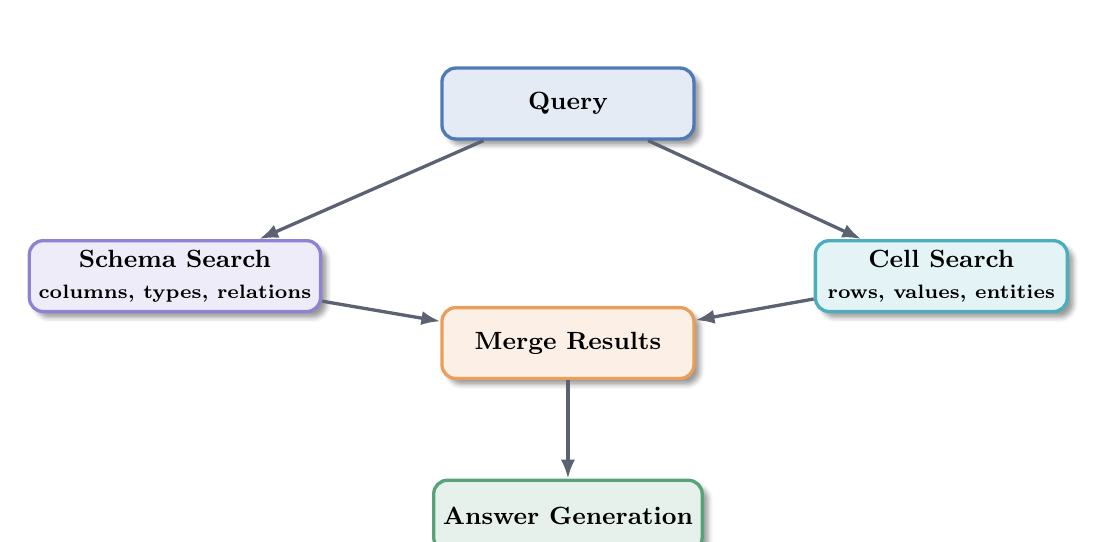
\begin{tikzpicture}[node distance=1.25cm and 1.5cm]
\node[block=prismblue] (query) {Query};
\node[block=prismpurple,below left=of query] (schema) {Schema Search\\\scriptsize columns, types, relations};
\node[block=prismcyan,below right=of query] (cells) {Cell Search\\\scriptsize rows, values, entities};
\node[block=prismorange,below=2.1cm of query] (merge) {Merge Results};
\node[block=prismgreen,below=of merge] (answer) {Answer Generation};
\draw[arrow] (query) -- (schema);
\draw[arrow] (query) -- (cells);
\draw[arrow] (schema) -- (merge);
\draw[arrow] (cells) -- (merge);
\draw[arrow] (merge) -- (answer);
\end{tikzpicture}
\caption{TableRAG combines schema and value indexes.}
\end{figure}

The schema index stores column names, descriptions, data types, and relationships. The
value index stores actual rows and cell values such as \texttt{PM Kisan},
\texttt{Karnataka}, \texttt{Rs. 6000}, and \texttt{Small Farmers}.

\section{Goal 7: Hierarchical Structure-Aware RAG}

\subsection{Objective}
Preserve document hierarchy during indexing for PDFs and Markdown documents.

\begin{figure}[h]
\centering
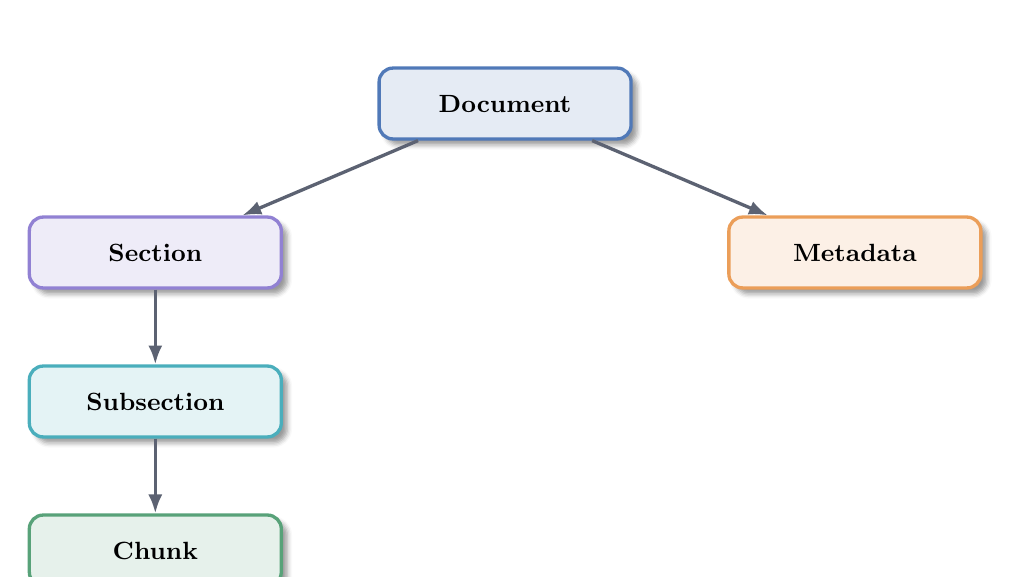
\begin{tikzpicture}[node distance=0.95cm and 1.2cm]
\node[block=prismblue] (doc) {Document};
\node[block=prismpurple,below left=of doc] (section) {Section};
\node[block=prismcyan,below=of section] (subsection) {Subsection};
\node[block=prismgreen,below=of subsection] (chunk) {Chunk};
\node[block=prismorange,below right=of doc] (metadata) {Metadata};
\draw[arrow] (doc) -- (section);
\draw[arrow] (section) -- (subsection);
\draw[arrow] (subsection) -- (chunk);
\draw[arrow] (doc) -- (metadata);
\end{tikzpicture}
\caption{Hierarchical index structure for PDF and Markdown retrieval.}
\end{figure}

The extraction layer identifies titles, chapters, sections, subsections, tables, lists,
and references. Retrieval proceeds from section to subsection to chunk before answer
generation.

\section{Goal 9: Agentic Retrieval Architecture}

\subsection{Objective}
Use specialized agents instead of a single monolithic retrieval chain.

\begin{longtable}{>{\bfseries}p{0.20\textwidth}p{0.50\textwidth}p{0.21\textwidth}}
\toprule
Agent & Responsibilities & Main Tools \\
\midrule
SQLite Agent & Query schemes database, generate SQL, aggregate results, return structured answers. & SQLite, schema explorer, SQL generator \\
Vector Retrieval Agent & Run ChromaDB search, query expansion, metadata filtering, similarity search, reranking, and context assembly. & ChromaDB, embeddings, reranker \\
Document Routing Agent & Select which documents should be searched before vector retrieval. & Registry, metadata filters \\
Web Enrichment Agent & Retrieve additional context when local data is insufficient. & Official portals, site extraction, verification \\
Retrieval Evaluation Agent & Evaluate coverage, confidence, source agreement, and completeness. & Scorers, policy rules \\
Coordinator Agent & Receive query, determine intent, invoke agents, merge results, generate final answer. & Agent orchestration \\
\bottomrule
\caption{Specialized retrieval agents.}
\end{longtable}

\subsection{Vector Query Expansion Example}
Input query: \texttt{PM Kisan Karnataka eligibility}. Expanded query terms include
\texttt{PM Kisan}, \texttt{Pradhan Mantri Kisan Samman Nidhi}, \texttt{Farmer Income
Support}, and \texttt{Eligibility Karnataka}.

\begin{lstlisting}[caption={Example vector retrieval result.}]
{
  "filename": "pm_kisan_guidelines.pdf",
  "section": "Eligibility",
  "score": 0.94
}
\end{lstlisting}

\section{Goal 10: Hybrid Retrieval Layer}

\subsection{Objective}
Combine SQL retrieval, vector search, TableRAG, metadata search, BM25 keyword search,
and web retrieval.

\begin{figure}[h]
\centering
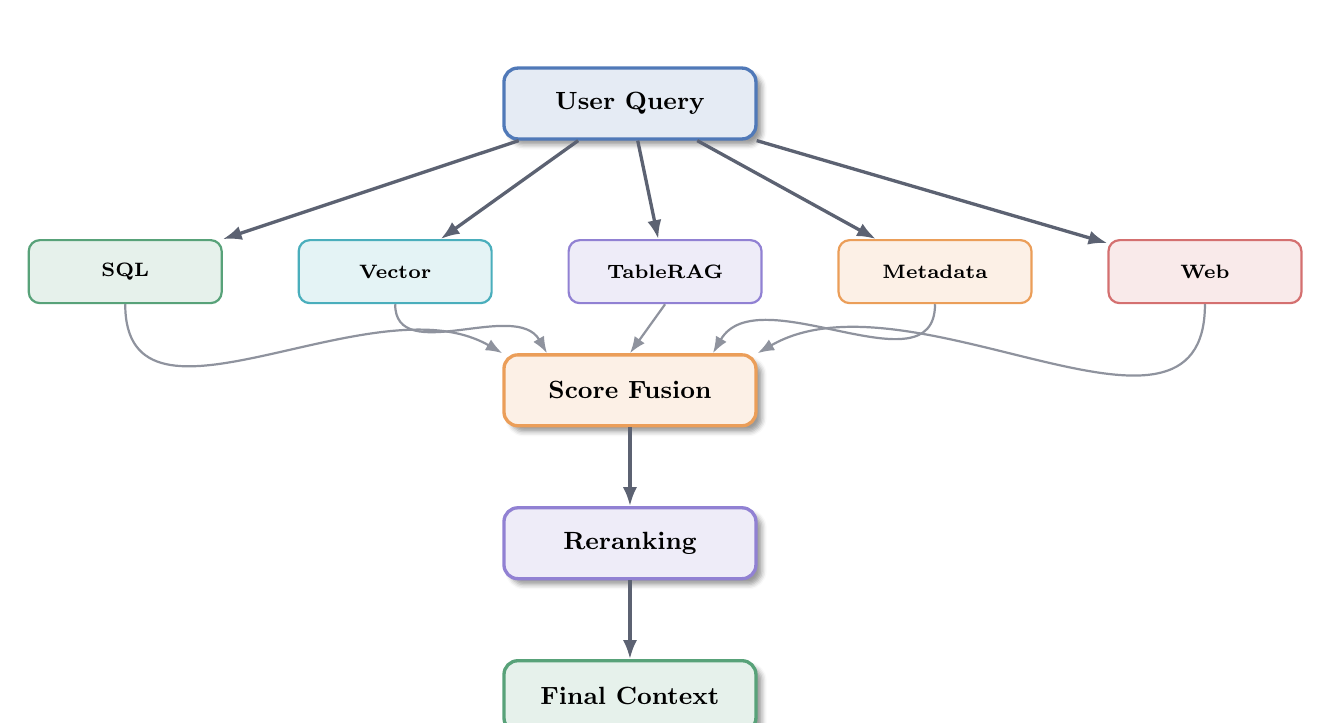
\begin{tikzpicture}[node distance=1cm and 0.95cm]
\node[block=prismblue] (query) {User Query};
\node[smallblock=prismgreen,below left=1.25cm and 3.55cm of query] (sql) {SQL};
\node[smallblock=prismcyan,right=of sql] (vector) {Vector};
\node[smallblock=prismpurple,right=of vector] (table) {TableRAG};
\node[smallblock=prismorange,right=of table] (metadata) {Metadata};
\node[smallblock=prismred,right=of metadata] (web) {Web};
\node[block=prismorange,below=2.7cm of query] (fusion) {Score Fusion};
\node[block=prismpurple,below=of fusion] (rerank) {Reranking};
\node[block=prismgreen,below=of rerank] (context) {Final Context};
\draw[arrow] (query) -- (sql);
\draw[arrow] (query) -- (vector);
\draw[arrow] (query) -- (table);
\draw[arrow] (query) -- (metadata);
\draw[arrow] (query) -- (web);
\draw[faintarrow] (sql.south) to[out=-90,in=150] (fusion.north west);
\draw[faintarrow] (vector.south) to[out=-90,in=120] ($(fusion.north west)!0.35!(fusion.north)$);
\draw[faintarrow] (table.south) -- (fusion.north);
\draw[faintarrow] (metadata.south) to[out=-90,in=60] ($(fusion.north east)!0.35!(fusion.north)$);
\draw[faintarrow] (web.south) to[out=-90,in=30] (fusion.north east);
\draw[arrow] (fusion) -- (rerank);
\draw[arrow] (rerank) -- (context);
\end{tikzpicture}
\caption{Hybrid retrieval and fusion layer.}
\end{figure}

\section{Goal 11: Reranking and Context Optimization}

\subsection{Objective}
Improve retrieval precision before generation.

\begin{figure}[h]
\centering
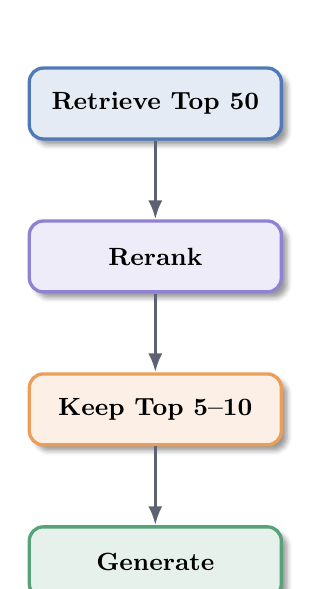
\begin{tikzpicture}[node distance=1cm]
\node[block=prismblue] (top) {Retrieve Top 50};
\node[block=prismpurple,below=of top] (rerank) {Rerank};
\node[block=prismorange,below=of rerank] (keep) {Keep Top 5--10};
\node[block=prismgreen,below=of keep] (generate) {Generate};
\draw[arrow] (top) -- (rerank);
\draw[arrow] (rerank) -- (keep);
\draw[arrow] (keep) -- (generate);
\end{tikzpicture}
\caption{Context optimization pipeline.}
\end{figure}

Core features include duplicate removal, distractor detection, relevance scoring, and
metadata weighting.

\newpage
\section{Complete System Architecture}

\begin{figure}[h]
\centering
\resizebox{\textwidth}{!}{%
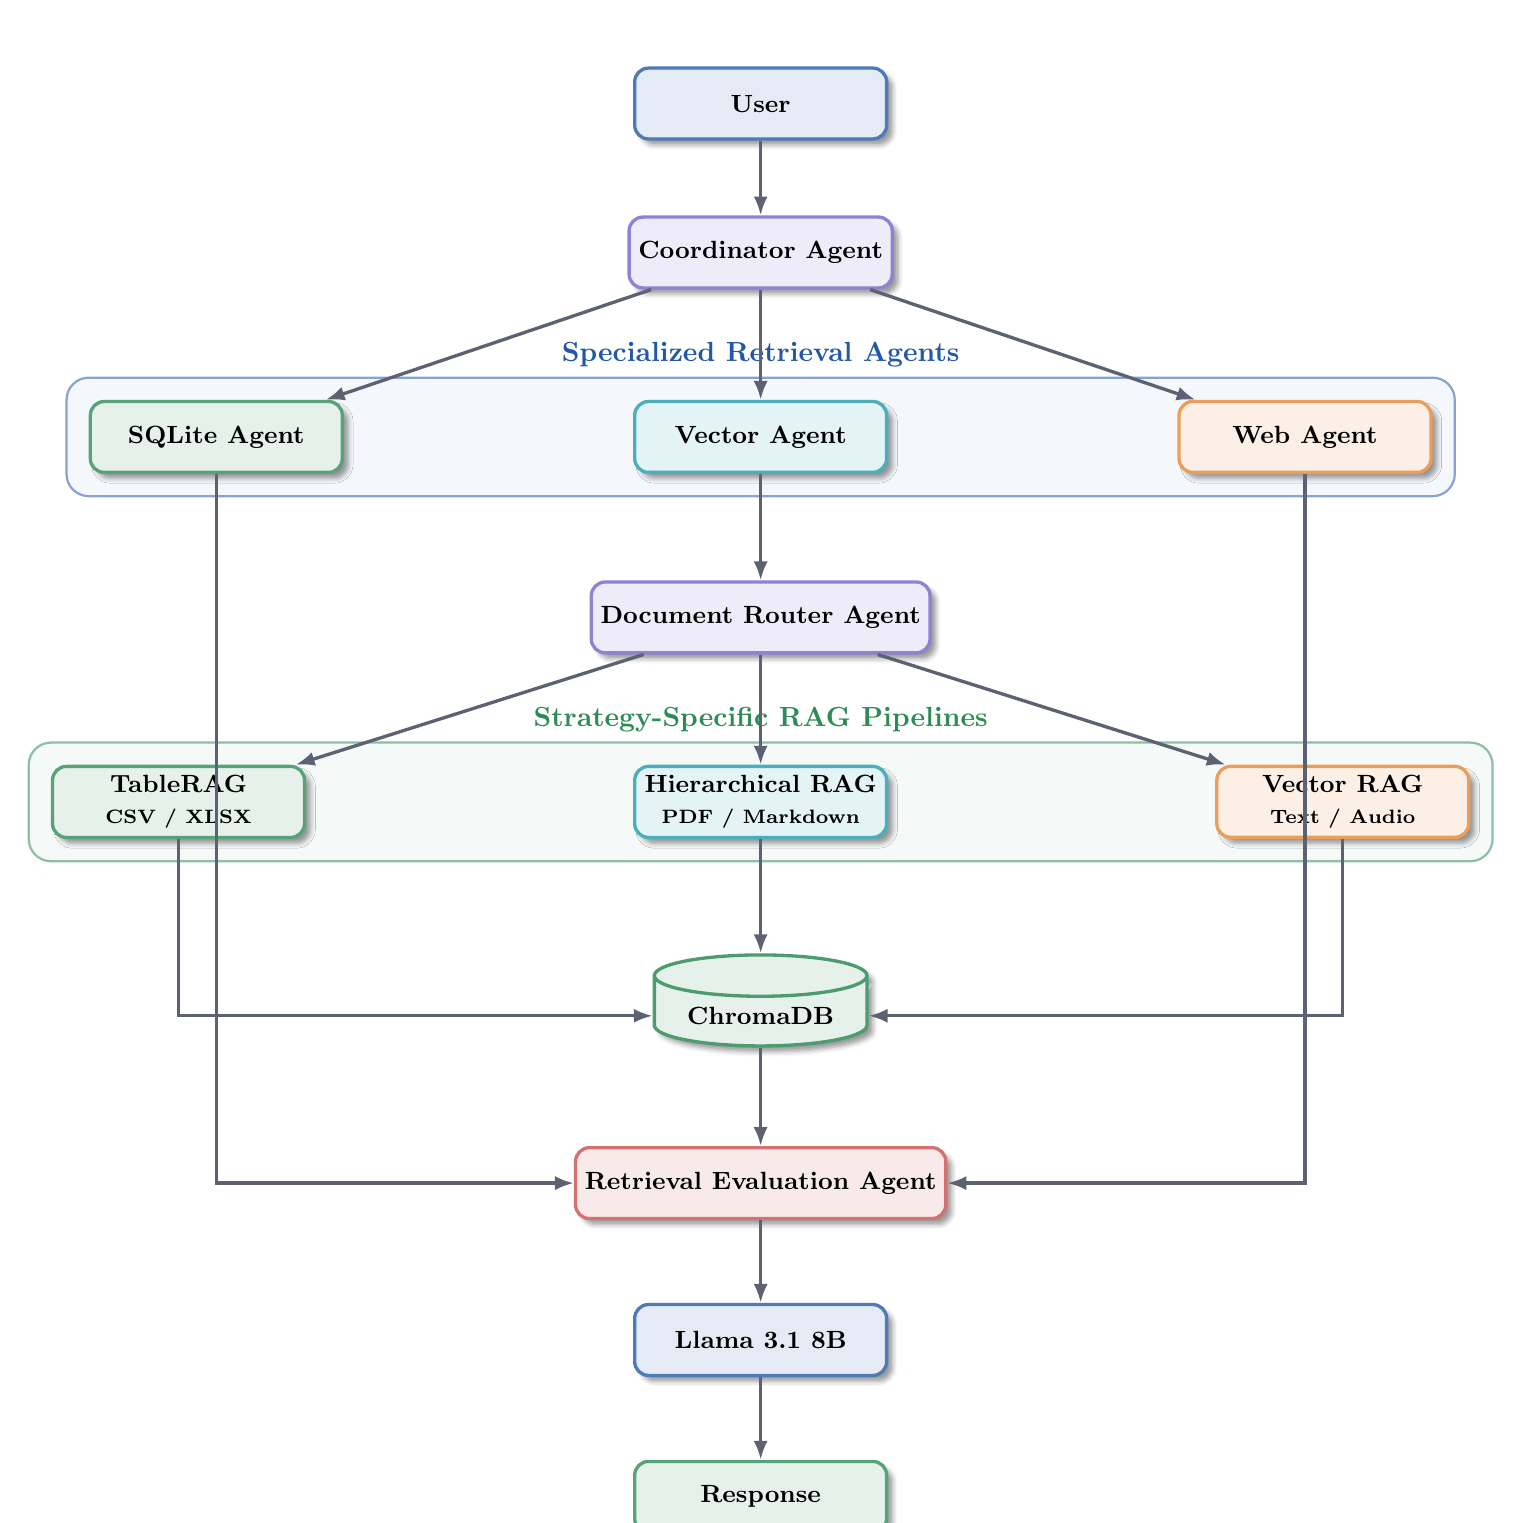
\begin{tikzpicture}[node distance=0.95cm and 1.0cm]
\node[block=prismblue] (user) {User};
\node[block=prismpurple,below=of user] (coord) {Coordinator Agent};

\node[block=prismgreen,below left=1.4cm and 3.6cm of coord] (sqlite) {SQLite Agent};
\node[block=prismcyan,below=1.4cm of coord] (vector) {Vector Agent};
\node[block=prismorange,below right=1.4cm and 3.6cm of coord] (web) {Web Agent};

\node[block=prismpurple,below=1.35cm of vector] (router) {Document Router Agent};

\node[block=prismgreen,below left=1.4cm and 3.6cm of router] (tablerag) {TableRAG\\\scriptsize CSV / XLSX};
\node[block=prismcyan,below=1.4cm of router] (hier) {Hierarchical RAG\\\scriptsize PDF / Markdown};
\node[block=prismorange,below right=1.4cm and 3.6cm of router] (vrag) {Vector RAG\\\scriptsize Text / Audio};

\node[store=prismgreen,below=1.45cm of hier] (chroma) {ChromaDB};
\node[block=prismred,below=1.25cm of chroma] (eval) {Retrieval Evaluation Agent};
\node[block=prismblue,below=1.05cm of eval] (llm) {Llama 3.1 8B};
\node[block=prismgreen,below=1.05cm of llm] (response) {Response};

\draw[arrow] (user) -- (coord);
\draw[arrow] (coord) -- (sqlite);
\draw[arrow] (coord) -- (vector);
\draw[arrow] (coord) -- (web);
\draw[arrow] (vector) -- (router);
\draw[arrow] (sqlite) |- (eval);
\draw[arrow] (web) |- (eval);
\draw[arrow] (router) -- (tablerag);
\draw[arrow] (router) -- (hier);
\draw[arrow] (router) -- (vrag);
\draw[arrow] (tablerag) |- (chroma);
\draw[arrow] (hier) -- (chroma);
\draw[arrow] (vrag) |- (chroma);
\draw[arrow] (chroma) -- (eval);
\draw[arrow] (eval) -- (llm);
\draw[arrow] (llm) -- (response);

\begin{scope}[on background layer]
  \node[group=prismblue,fit=(sqlite)(vector)(web),label={[font=\bfseries\color{prismblue}]above:Specialized Retrieval Agents}] {};
  \node[group=prismgreen,fit=(tablerag)(hier)(vrag),label={[font=\bfseries\color{prismgreen}]above:Strategy-Specific RAG Pipelines}] {};
\end{scope}
\end{tikzpicture}%
}
\caption{End-to-end agentic multimodal RAG architecture.}
\end{figure}

\section{Implementation Milestones}

\begin{enumerate}
  \item Normalize the government schemes database and expose the initial SQLite-backed API.
  \item Build the document registry and metadata validation rules.
  \item Implement upload detection, document routing, and strategy selection.
  \item Add TableRAG, hierarchical RAG, and vector RAG indexing pipelines.
  \item Integrate ChromaDB collections, metadata filtering, and multi-collection search.
  \item Add agent orchestration, retrieval evaluation, reranking, and web enrichment.
  \item Ship frontend views for schemes, uploaded documents, sources, and final answers.
\end{enumerate}

\end{document}
